\documentclass[12pt,a4paper]{article}
\usepackage{vntex} % Tiếng Việt
\usepackage{graphicx} % Chèn hình ảnh
\usepackage{listings} % Thêm gói listings để chèn code
\usepackage{xcolor} % Màu cho code
\usepackage{changepage} % Thay đổi lề
\lstset{
    language=R,
    basicstyle=\footnotesize\ttfamily,
    numbers=none,
    numberstyle=\tiny\color{gray},
    stepnumber=1,
    numbersep=0.01pt,
    tabsize=2,
    breaklines=true,
    breakatwhitespace=false,
    xleftmargin=0cm, % for line numbers
    framexleftmargin=0cm, % for code frame
    keywordstyle=\color{blue},
    commentstyle=\color{green},
    stringstyle=\color{orange},
    frame=single,
    rulecolor=\color{black},
    basicstyle=\ttfamily,
}
% Thiết lập bảng
\usepackage{diagbox}
\usepackage{array}
\usepackage{tabularx}
\usepackage{longtable} % Tạo bảng qua nhiều trang
\usepackage{cellspace}
\usepackage{bm} % Chữ in đậm trong công thức toán 
\usepackage{a4wide,amssymb,epsfig,latexsym,multicol,array,hhline,fancyhdr}
\usepackage{tikz}
\usepackage{color}
\usepackage{subcaption}
\usepackage{framed}
\usepackage{float} % Để chèn hình ảnh vào đúng vị trí
\usepackage{fancyvrb} %Đưa dữ liệu dạng nguyên thủy vào
\usepackage{amsmath} % Công thức toán
\usepackage{slashbox} % Chèn đường chéo trong bảng
% Thiết lập kích thước
\usepackage{geometry}
\geometry{
    left=3cm,
    right=2cm,
    top=2.5cm,
    bottom=2.5cm,
}
\usepackage{hyperref} %Chèn link
\hypersetup{urlcolor=black,linkcolor=black,citecolor=black,colorlinks=true} % Màu cho các đường nét
\everymath{\color{black}}
\setlength{\headheight}{40pt}
\pagestyle{fancy}


%Header
\fancyhead{} % clear all header fields
\fancyhead[L]{
 \begin{tabular}{rl}
    \begin{picture}(25,15)(0,0)
    \put(0,-8){
\includegraphics[width=12mm, height=12mm]{pictures/hcmut.png}}
    %\put(0,-8){\epsfig{width=10mm,figure=hcmut.eps}}
   \end{picture}&
	%
\includegraphics[width=8mm, height=8mm]{hcmut.png} & %
	\begin{tabular}{l}
		\textbf{\bf \ttfamily Trường Đại Học Bách Khoa - ĐHQG TP.Hồ Chí Minh}\\
		\textbf{\bf \ttfamily Khoa Cơ Khí - Bộ môn Cơ Điện Tử}
	\end{tabular} 	
 \end{tabular}
}
\fancyhead[R]{
	{\tiny \bf \quad} % Khoảng trắng nhỏ trong header bên phải
}

%Footer
\fancyfoot{} % clear all footer fields
\fancyfoot[L]{\scriptsize \ttfamily Trang bị điện - điện tử trong máy công nghiệp}
\fancyfoot[R]{\scriptsize \ttfamily Trang {\thepage}/11}
\renewcommand{\headrulewidth}{0.3pt}
\renewcommand{\footrulewidth}{0.3pt}

\begin{document}
    \begin{titlepage}   
    \begin{center}
        \vspace*{-2cm} 
        \large
        \textbf{ĐẠI HỌC QUỐC GIA THÀNH PHỐ HỒ CHÍ MINH \\
        TRƯỜNG ĐẠI HỌC BÁCH KHOA\\
        KHOA CƠ KHÍ\\
        BỘ MÔN CƠ ĐIỆN TỬ}\\
        
\includegraphics[width=70mm, height=70mm]{pictures/hcmut.png} \\
        \rule{\linewidth}{0.5mm}\\
        \vspace{0.8cm}
        \Large
        \textbf{TRANG BỊ ĐIỆN - ĐIỆN TỬ TRONG MÁY CÔNG NGHIỆP}\\
        \vspace*{0.5cm}
        \Huge
        \textbf{EXERCISE 4}\\
        \vspace{0.5cm}
        \rule{\linewidth}{0.5mm}\\
        \vspace{0.8cm}
        \vspace{1cm}
        \large
        GVHD: TS. LÊ ĐỨC HẠNH\\
        \vspace{0.5cm}
        DANH SÁCH THÀNH VIÊN:\\[0.3cm]
        \begin{tabular}{|>{\centering\arraybackslash}m{1cm}|>{\centering\arraybackslash}m{7cm}|>{\centering\arraybackslash}m{5cm}|}
            \hline
            \textbf{STT} & \textbf{Họ và tên} & \textbf{MSSV} \\
            \hline
            1 & Võ Hữu Dư & 2210604 \\
            \hline
            2 & Dương Quang Duy & 2210497 \\
            \hline
            3 & Trần Quang Đạo & 2210647 \\
            \hline
        \end{tabular}
    \end{center}
        
    \vfill
    \large
    \begin{center}
        TP.HCM, \today
    \end{center}
\end{titlepage}

	\tableofcontents
	\newpage
	\section{Design a control circuit for described operation below:}
\subsection{Push button start.}
\subsubsection{Motor 1 (AC1phase), Motor2(3phase) run in star mode, after 5s motor 1 change direction, motor 2 change from star to delta, motor 3 start running.}
Motor 1 (AC1phase), Motor 2 (3phase) run in star mode:
\begin{figure}[H]
    \centering
    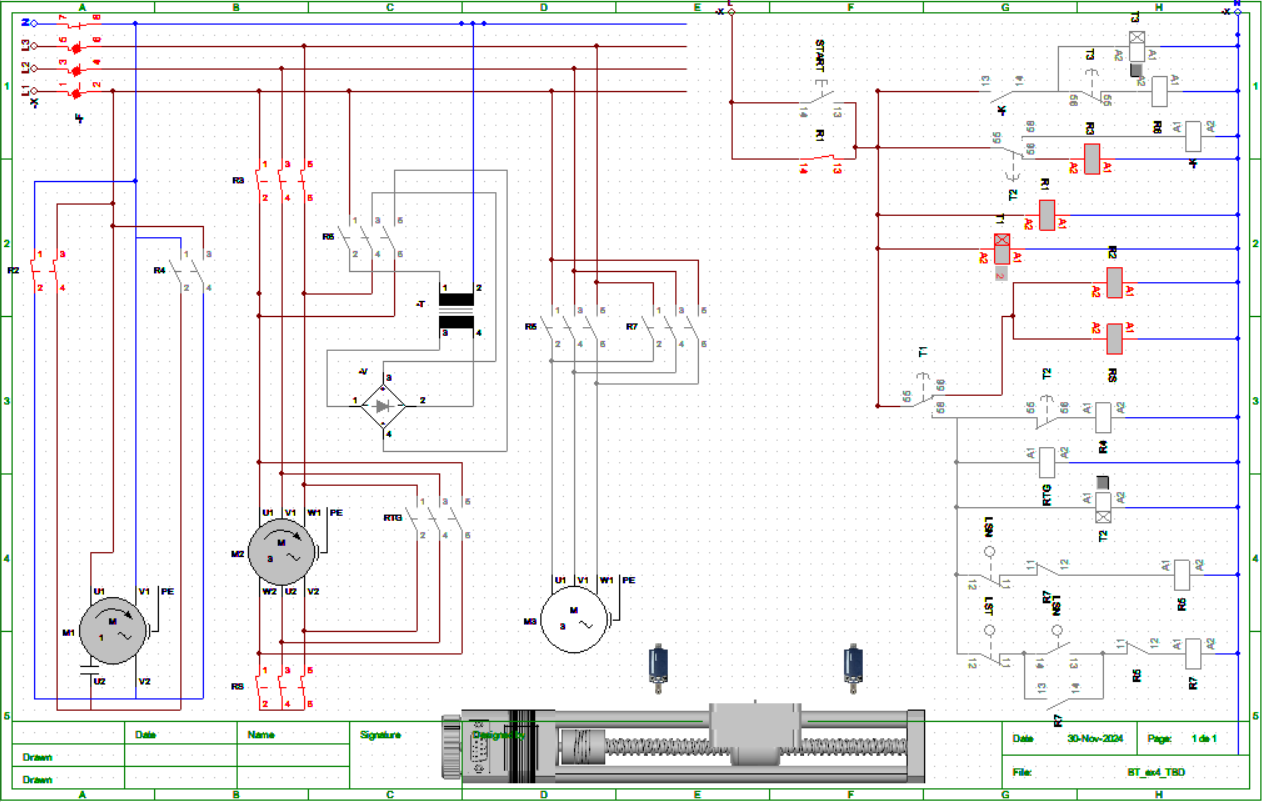
\includegraphics[width=1\textwidth]{pictures/1a.png}
\end{figure}
\cleardoublepage
After 5s motor 1 change direction, motor 2 change from star to delta, motor 3 start running:
\begin{figure}[H]
    \centering
    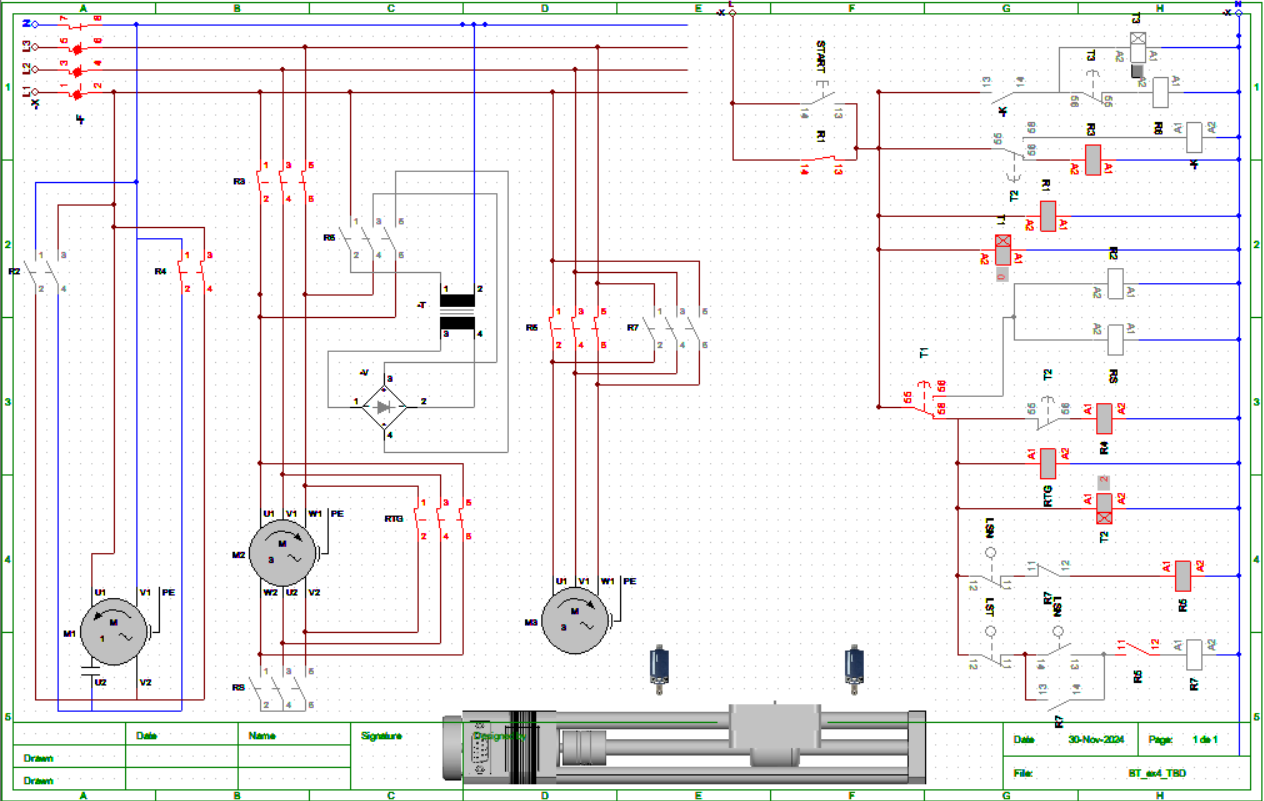
\includegraphics[width=1\textwidth]{pictures/1b.png}
\end{figure}
\cleardoublepage
\subsubsection{Motor 3 (3phase) runs from left to right then meets a limit switch then return to right then loop again,  while in 5s later motor1 stops and motor2 stop (kinematic).}
Motor 3 (3phase) runs from left to right then meets a limit switch then return to right then loop again:
\begin{figure}[H]
    \centering
    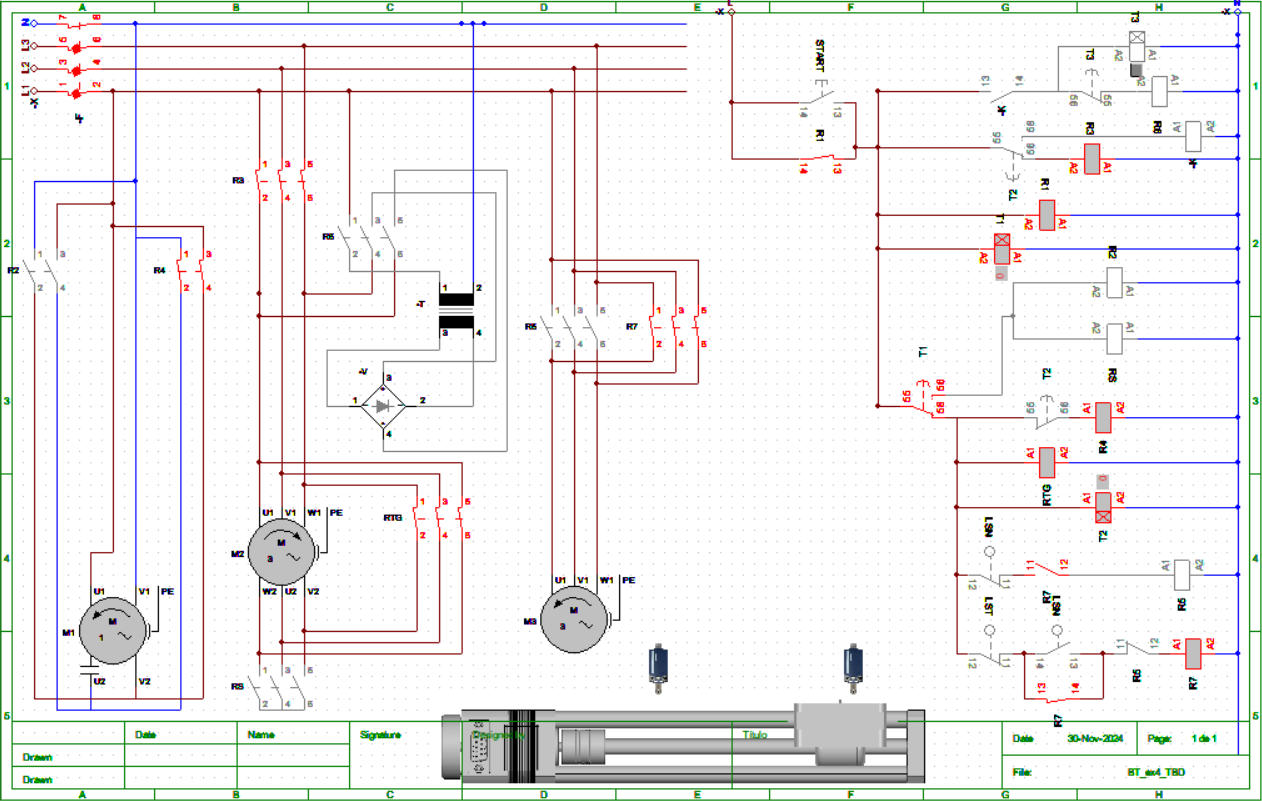
\includegraphics[width=1\textwidth]{pictures/1c.png}
\end{figure}
\cleardoublepage
In 5s later motor 1 stops and motor 2 stop (kinematic):
\begin{figure}[H]
    \centering
    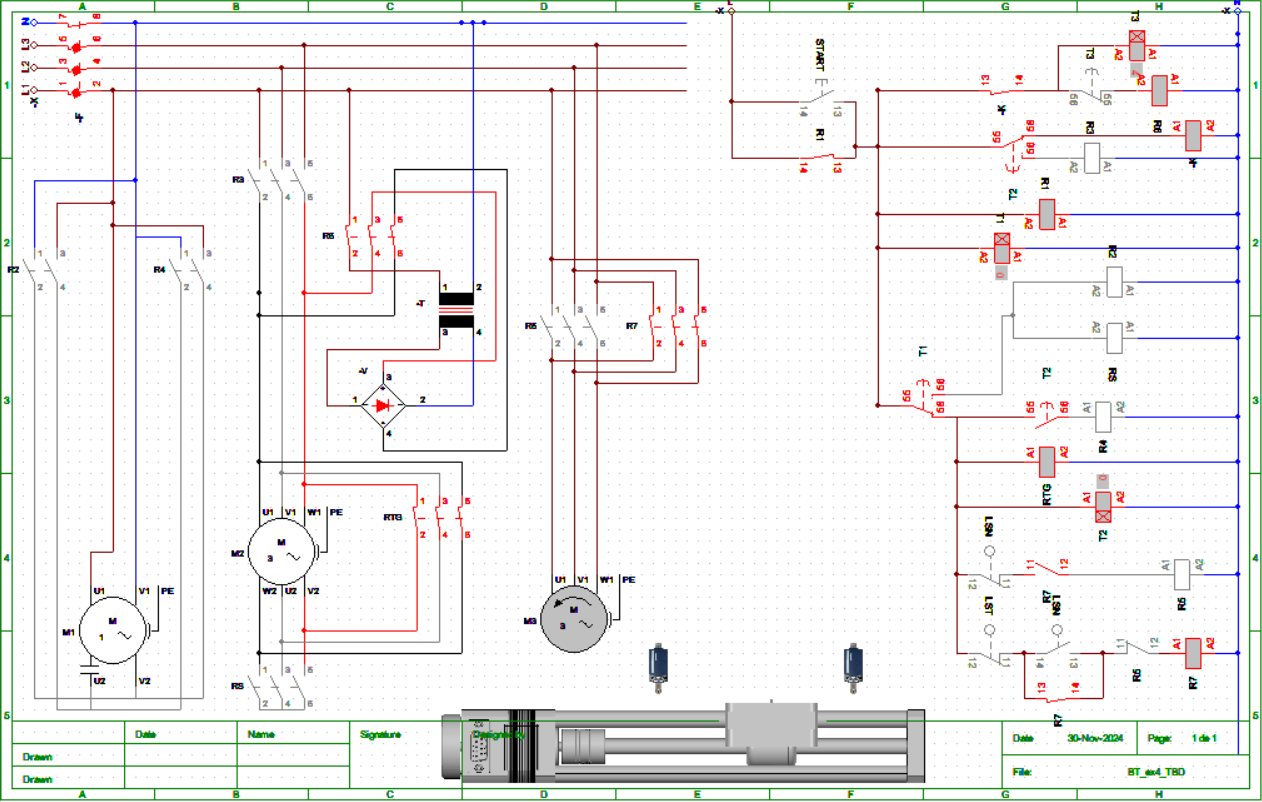
\includegraphics[width=1\textwidth]{pictures/1d.png}
\end{figure}
\cleardoublepage
\subsection{Circuit have emergency stop button.}
\subsubsection{Before the emergency stop button is pressed}
\begin{figure}[H]
    \centering
    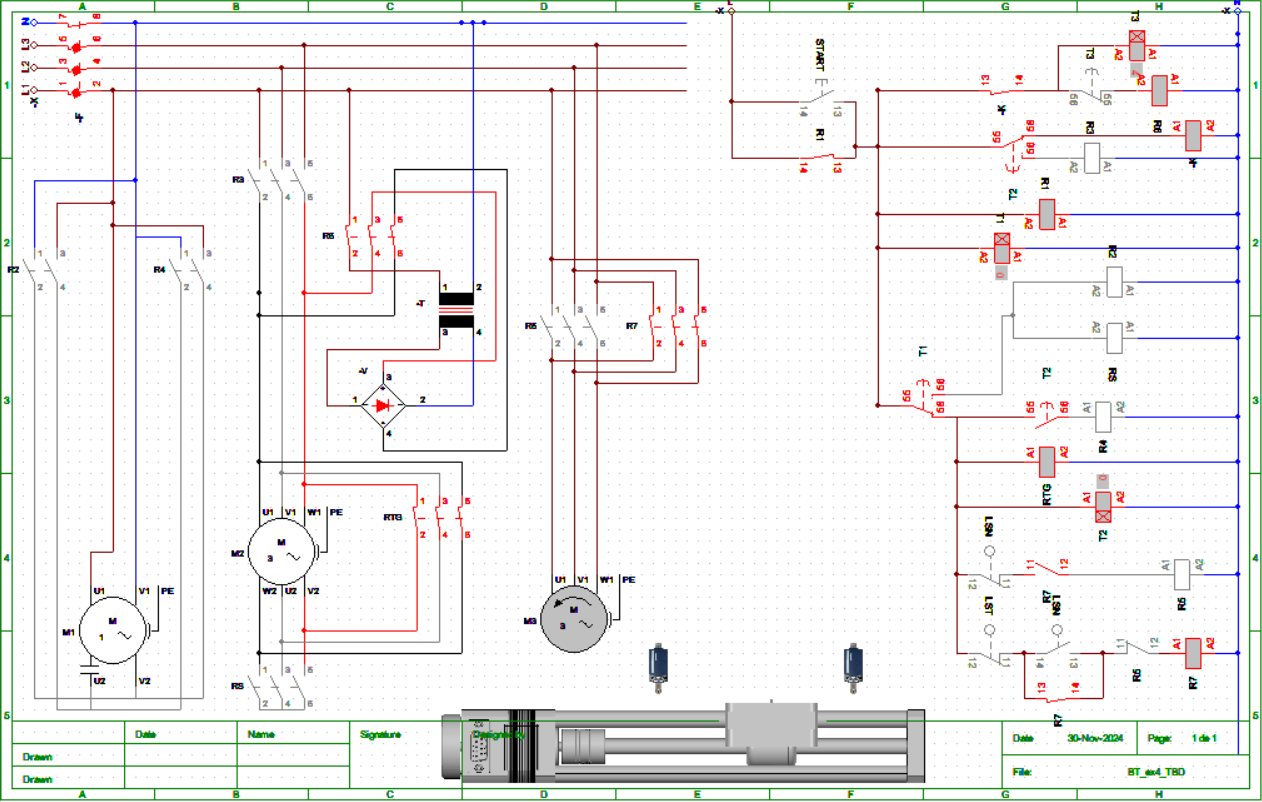
\includegraphics[width=1\textwidth]{pictures/1d.png}
\end{figure}
\cleardoublepage
\subsubsection{After the emergency stop button is pressed}
\begin{figure}[H]
    \centering
    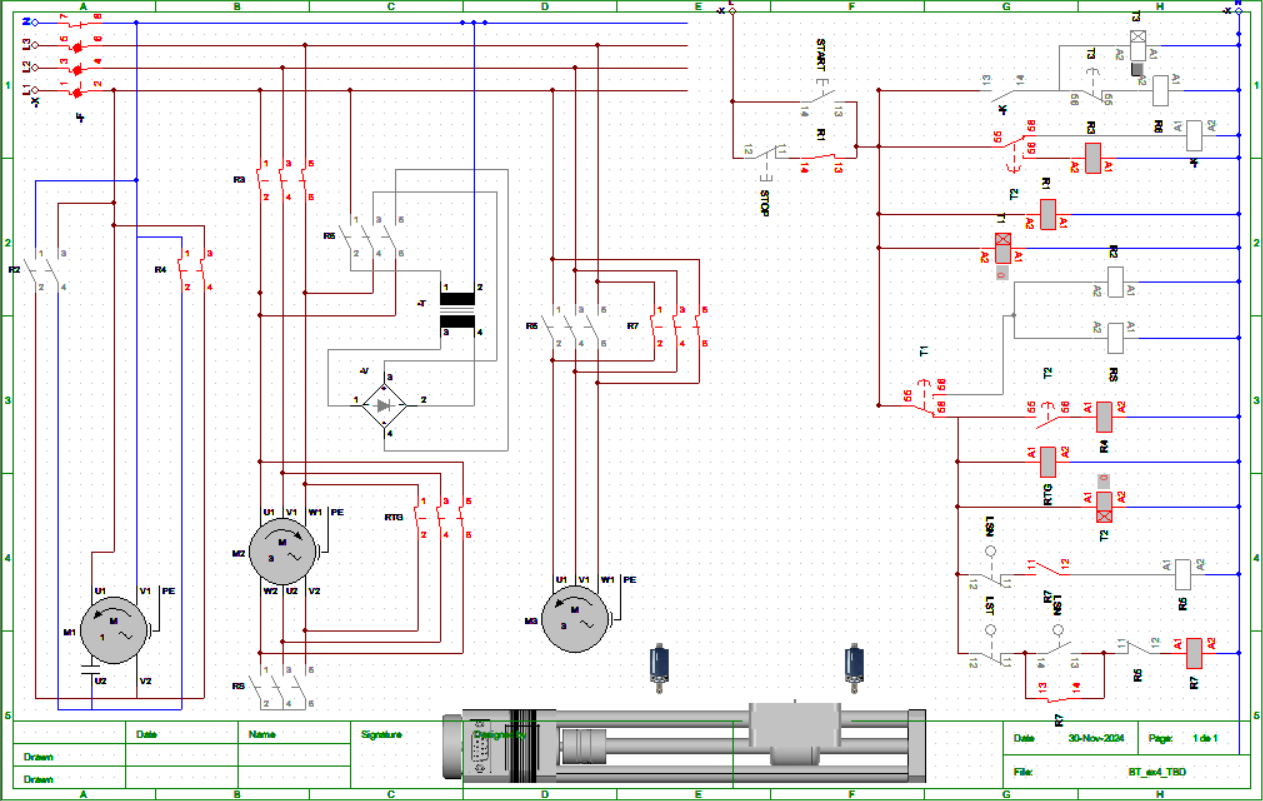
\includegraphics[width=1\textwidth]{pictures/1e.png}
\end{figure}
$\Rightarrow$ After the emergency stop button is pressed, all motors stop immediately and will not reactivate until the start button is pressed.
\cleardoublepage
	\section{Design the contactors, relays, fuse, lamp, wire, aptomat, for the circuit below:}
    \textbf{U=220V, Lathe machine (máy tiện), Milling machine (máy phay), punching machine (máy dập), Planning machine (máy bào), boiler machine (lò đun) use 3phase power, the remaining use AC 1 phase. Show detail information and picture selected electrical device.}
    \begin{figure}[H]
        \centering
        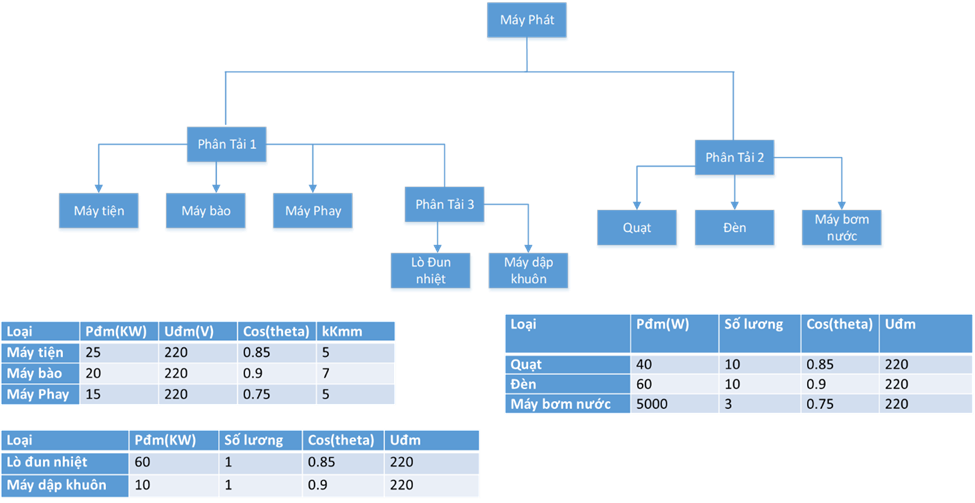
\includegraphics[width=1\textwidth]{pictures/2a.png}
    \end{figure}
    \subsection{Tính toán tải}
        \begin{itemize} 
            \item Cường độ dòng điện định mức trong hệ thống điện AC 1 pha:
                \begin{align}
                    I_{dm} = n \times \frac{S \times 1000}{U}
                \end{align}
            \item Cường độ dòng điện định mức trong hệ thống điện AC 3 pha:
                \begin{align}
                    I_{dm} = n \times \frac{S \times 1000}{U \times \sqrt{3}}
                \end{align}
            Trong đó:
            \begin{itemize}
                \item $S = \frac{P}{\cos(\theta)}$ là công suất biểu kiến của tải.
                \item $U$ là điện áp (V).
                \item $n$ là hệ số công suất.
             \end{itemize}
        \end{itemize}
        \subsubsection{Phần tải 1}
            \begin{itemize}
                \item Máy tiện: 
                    \begin{itemize}
                        \item $S = \frac{25}{0.85} = 29.4118 (kW)$
                        \item $I = \frac{29.4118 \times 1000}{220 \times \sqrt{3}} = 77.186 (A)$
                    \end{itemize}
                \item Máy bào: 
                    \begin{itemize}
                        \item $S = \frac{20}{0.9} = 22.2222 (kW)$
                        \item $I = \frac{22.2222 \times 1000}{220 \times \sqrt{3}} = 58.318 (A)$
                    \end{itemize}
                \item Máy phay:
                    \begin{itemize}
                        \item $S = \frac{15}{0.75} = 20 (kVA)$
                        \item $I = \frac{20 \times 1000}{220 \times \sqrt{3}} = 52.3864 (A)$
                    \end{itemize}
                \item Tổng cường độ dòng điện qua tải 1:
                    \begin{align*}
                        I_{1} = 77.186 + 58.318 + 52.3864 = 187.8904 (A)
                    \end{align*} 
            \end{itemize}
        \subsubsection{Phần tải 2}
            \begin{itemize}
                \item Quạt:
                    \begin{itemize}
                        \item $S = \frac{0.04}{0.85} = 0.047 (kW)$
                        \item $I = 10 \times \frac{0.047 \times 1000}{220} = 2.14 (A)$
                    \end{itemize}
                \item Đèn:
                    \begin{itemize}
                        \item $S = \frac{0.06}{0.9} = 0.0667 (kVA)$
                        \item $I = 10 \times \frac{0.0667 \times 1000}{220} = 3.0318 (A)$
                    \end{itemize}
                \item Máy bơm nước:
                    \begin{itemize}
                        \item $S = \frac{5}{0.75} = 6.6667 (kW)$
                        \item $I = 3 \times \frac{6.6667 \times 1000}{220} = 90.9095 (A)$
                    \end{itemize}
                \item Tổng cường độ dòng điện phần tải 2:
                    \begin{align*}
                        I_{2} = 2.14 + 3.0318 + 90.9095 = 96.0813 (A)
                    \end{align*}
            \end{itemize}
        \subsubsection{Phần tải 3}
            \begin{itemize}
                \item Lò đun:
                    \begin{itemize}
                        \item $S = \frac{60}{0.85} = 70.5882 (kW)$
                        \item $I = 1 \times \frac{70.5882 \times 1000}{220 \times \sqrt{3}} = 185.246 (A)$
                    \end{itemize}
                \item Máy dập khuôn:
                    \begin{itemize}
                        \item $S = \frac{10}{0.9} = 11.1111 (kW)$
                        \item $I = 1 \times \frac{11.1111 \times 1000}{220 \times \sqrt{3}} = 29.159 (A)$
                    \end{itemize}
                \item Tổng cường độ dòng điện phần tải 3:
                    \begin{align*}
                        I_{3} = 185.246 + 29.159 = 214.405 (A)
                    \end{align*}
            \end{itemize}
        \textbf{Tổng cường độ dòng điện qua toàn bộ hệ thống:}
        \begin{align*}
            I = 187.8904 + 96.0813 + 214.405 = 498.3767 (A)
        \end{align*}
    \subsection{Chọn thiết bị}
        \subsubsection{Contactor và Relay nhiệt}
            \textbf{Điều kiện chọn contactor và relay nhiệt:}
                \begin{itemize}
                    \item Chọn contactor và relay nhiệt có $I = 1.2 \div 1.4 \times I_{dm} (A)$.
                    \item Chọn contactor và relay nhiệt có $U = 220 (V)$.
                \end{itemize}
            \textbf{Chọn contactor và relay nhiệt cho tải 1}     
                \begin{itemize}
                    \item Dòng điện contactor: $I_{ct} = 1.3 \times I_{1} = 244.2575$
                    \item Điện áp hoạt động: 220V.\\[0.2cm]
                        $\Rightarrow$ \textbf{Ta chọn được Contactor Mitsubishi S-N220 250A 2NO+2NC 220V và Rơ le nhiệt Mitsubishi TH-N220KPRH 210A (170-250A)}.
                        \begin{figure}[H]
                            \centering
                            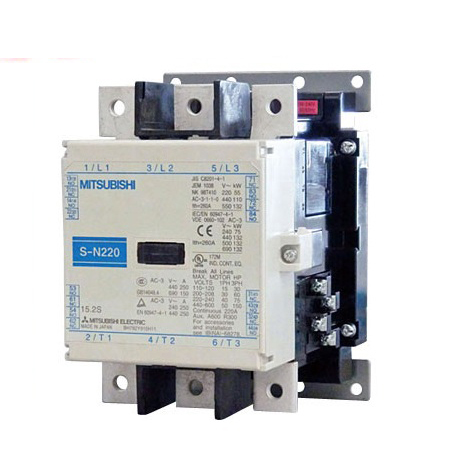
\includegraphics[width=0.4\textwidth]{pictures/2b1.png}
                            \caption{Contactor Mitsubishi S-N220 250A 2NO+2NC 220V}
                        \end{figure}
                        \begin{figure}[H]
                            \centering
                            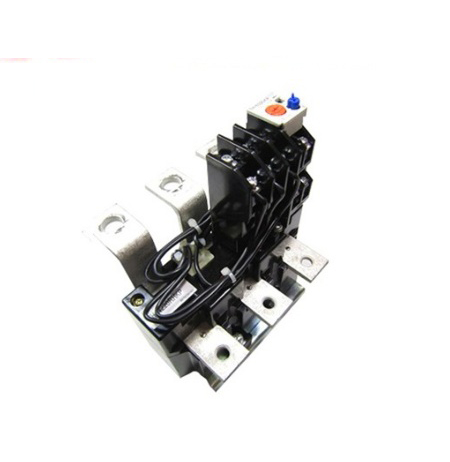
\includegraphics[width=0.4\textwidth]{pictures/2b2.png}
                            \caption{Rơ le nhiệt Mitsubishi TH-N220KPRH 210A (170-250A)}
                        \end{figure}
                    \item Thông số kỹ thuật contactor:
                        \begin{itemize}
                            \item Thương hiệu: Mitsubishi.
                            \item Điện áp: 220V.
                            \item Dòng định mức: 250A.
                            \item Công suất: 132kW.
                            \item Tiếp điểm: 2NC + 2NO.
                            \item Series: Mitsubishi S-N.
                            \item Đường dẫn sản phẩm: \href{https://codienhaiau.com/product/cong-tac-to-dang-khoi-mitsubishi-s-n220-ac200v/}{Contactor Mitsubishi}.
                        \end{itemize}
                    \item Thông số kỹ thuật relay nhiệt:
                        \begin{itemize}
                            \item Thương hiệu: Mitsubishi.
                            \item Dòng định mức: 250A.
                            \item Dãi điều chỉnh: 170-250A.
                            \item Series: Mitsubishi TH-N.
                            \item Đường dẫn sản phẩm: \href{https://codienhaiau.com/product/ro-le-nhiet-mitsubishi-th-n220kprh-210a/}{Rơ le nhiệt Mitsubishi}.
                        \end{itemize}
                \end{itemize}
            \textbf{Chọn contactor và relay nhiệt cho tải 2}
                \begin{itemize}
                    \item Dòng điện contactor: $I_{ct} = 1.3 \times I_{2} = 124.90569$
                    \item Điện áp hoạt động: 220V.\\[0.2cm]
                        $\Rightarrow$ \textbf{Ta chọn được Contactor LS MC-130a 220V 130A 60kW 2NC+2NO và Rơ le nhiệt LS MT-150 (95-130A).}
                        \begin{figure}[H]
                            \centering
                            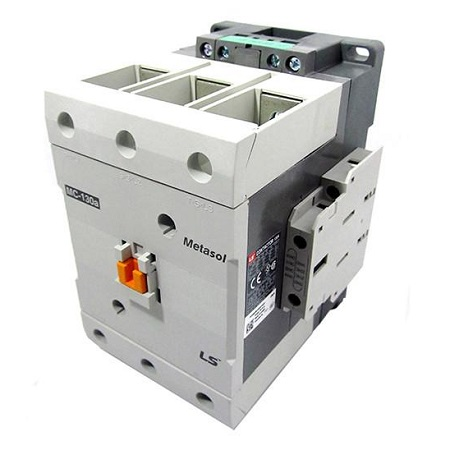
\includegraphics[width=0.4\textwidth]{pictures/2c1.png}
                            \caption{Contactor LS MC-130a 220V 130A 60kW 2NC+2NO}
                        \end{figure}
                        \begin{figure}[H]
                            \centering
                            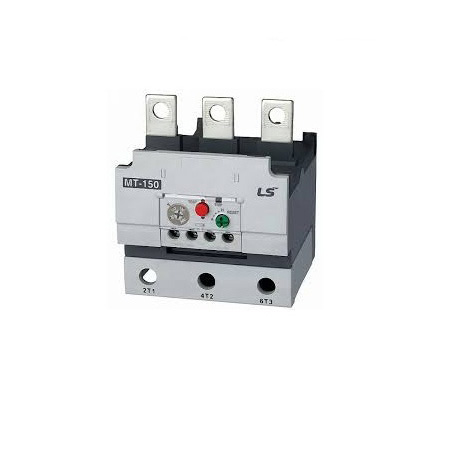
\includegraphics[width=0.4\textwidth]{pictures/2c2.png}
                            \caption{Rơ le nhiệt LS MT-150 (95-130A)}
                        \end{figure}
                    \item Thông số kỹ thuật contactor:
                        \begin{itemize}
                            \item Thương hiệu: LS.
                            \item Điện áp: 380V.
                            \item Dòng định mức: 130A.
                            \item Công suất: 60kW.
                            \item Tiếp điểm: 2NC + 2NO.
                            \item Series: LS MC.
                            \item Đường dẫn sản phẩm: \href{https://codienhaiau.com/product/contactor-ls-mc-130a-60kw-2no2nc-coil-380v/}{Contactor LS}.
                        \end{itemize}
                    \item Thông số kỹ thuật relay nhiệt:
                        \begin{itemize}
                            \item Thương hiệu: LS.
                            \item Dòng định mức: 130A.
                            \item Dãi điều chỉnh: 95-130A.
                            \item Series: LS MT.
                            \item Đường dẫn sản phẩm: \href{https://codienhaiau.com/product/ro-le-nhiet-ls-mt-150-95-130a/}{Rơ le nhiệt LS}.
                        \end{itemize}
                \end{itemize}
            \textbf{Chọn contactor và relay nhiệt cho tải 3}
                \begin{itemize}
                    \item Dòng điện contactor: $I_{ct} = 1.3 \times I_{3} = 278.7265 $ 
                    \item Điện áp hoạt động: 220V.\\[0.2cm]
                        $\Rightarrow$ \textbf{Ta chọn được Contactor Schneider LC1D65AM7 3P 65A 220V và Rơ le nhiệt Mitsubishi TH-N600KP 250A (200-300A)}
                        \begin{figure}[H]
                            \centering
                            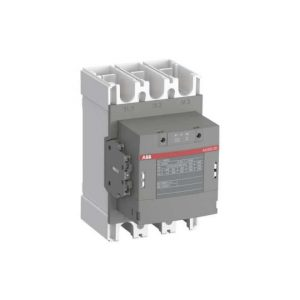
\includegraphics[width=0.4\textwidth]{pictures/2d1.png}
                            \caption{Contactor ABB AX300-30-11-88 300A 160kW 230-240V}
                        \end{figure}
                        \begin{figure}[H]
                            \centering
                            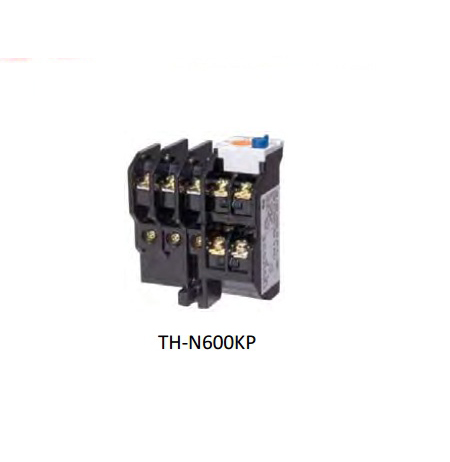
\includegraphics[width=0.4\textwidth]{pictures/2d2.png}
                            \caption{Rơ le nhiệt Mitsubishi TH-N600KP 250A (200-300A)}
                        \end{figure}
                    \item Thông số kỹ thuật contactor:
                        \begin{itemize}
                            \item Thương hiệu: ABB.
                            \item Trọng lượng: 4.7kg.
                            \item Kích thước: 18x14x22.5cm.
                            \item Điện áp: 220V.
                            \item Dòng định mức: 300A.
                            \item Công suất: 160kW.
                            \item Tiếp điểm phụ: 1NC + 1NO.
                            \item Đường dẫn sản phẩm: \href{https://codienhaiau.com/product/1sfl587074r8811/}{Contactor ABB}.
                        \end{itemize}
                    \item Thông số kỹ thuật relay nhiệt:
                        \begin{itemize}
                            \item Thương hiệu: Mitsubishi.
                            \item Dòng định mức: 250A.
                            \item Dãi điều chỉnh: 200-300A.
                            \item Series: Mitsubishi TH-N.
                            \item Đường dẫn sản phẩm: \href{https://codienhaiau.com/product/ro-le-nhiet-mitsubishi-th-n600kp-250a/}{Rơ le nhiệt Mitsubishi}.
                        \end{itemize}
                \end{itemize}
        \subsubsection{Fuses}
            \textbf{Điều kiện chọn cầu chì}
                \begin{itemize}
                    \item Chọn cầu chì có $I = 1.5 \times I_{dm} (A)$.
                \end{itemize}
            \textbf{Chọn cầu chì cho tải 1}
                \begin{itemize}
                    \item Dòng điện cầu chì: $I_{f} = 1.5 \times I_{1} = 281.8356A$ \\[0.2cm]
                        $\Rightarrow$ \textbf{Ta chọn được Cầu chì Omega 300A NH2S 500VAC gG 120kA}.
                        \begin{figure}[H]
                            \centering
                            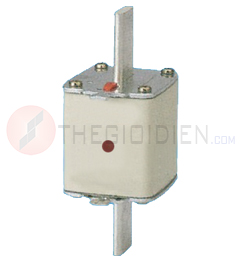
\includegraphics[width=0.3\textwidth]{pictures/2e.png}
                            \caption{Cầu chì Omega 300A NH2S 500VAC gG 120kA}
                        \end{figure}
                    \item Thông số kỹ thuật cầu chì:
                        \begin{itemize}
                            \item Thương hiệu: Omega.
                            \item Dòng định mức: 300A 500V AC.
                            \item Dòng ngắn mạch: 120kA.
                            \item Kích thước: NH2S.
                            \item Báo trạng thái ngắt mạch: Có.
                            \item Đường dẫn sản phẩm: \href{https://www.thegioidien.com/sanpham/5/20817/Cau-chi-300A-NH2S-500VAC-gG-120kA.aspx}{Cầu chì Omega}.
                        \end{itemize}
                \end{itemize}
            \textbf{Chọn cầu chì cho tải 2}
                \begin{itemize}
                    \item Dòng điện cầu chì: $I_{f} = 1.5 \times I_{2} = 144.12195A$ \\[0.2cm]
                        $\Rightarrow$ \textbf{Ta chọn được Cầu chì LS HRC 160A 220V}.
                        \begin{figure}[H]
                            \centering
                            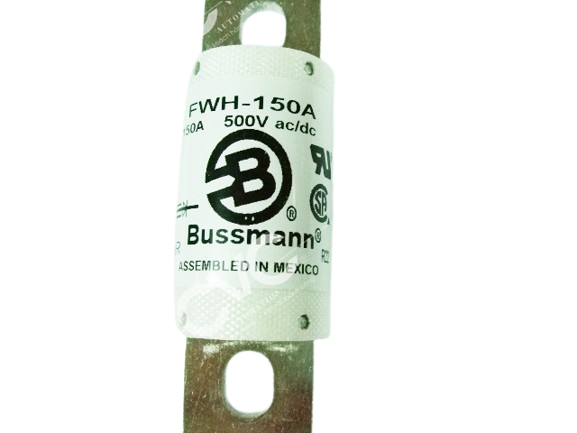
\includegraphics[width=0.3\textwidth]{pictures/2f.png}
                            \caption{Cầu chì Bussmann FWH-150A}
                        \end{figure}
                    \item Thông số kỹ thuật cầu chì:
                        \begin{itemize}
                            \item Thương hiệu: Bussman.
                            \item Dòng định mức: 150A.
                            \item Dòng ngắn mạch: 200kA.
                            \item Kích thước: khoảng cách 2 tâm lỗ 71mm-75mm.
                            \item Báo trạng thái ngắt mạch: Không.
                            \item Đường dẫn sản phẩm: \href{https://www.chauvinhcuong.com/cau-chi--bussmann-fwh-150a}{Cầu chì Bussman}.
                        \end{itemize}
                \end{itemize}
            \textbf{Chọn cầu chì cho tải 3}
                \begin{itemize}
                    \item Dòng điện cầu chì: $I_{f} = 1.5 \times I_{3} = 321.6075A$ \\[0.2cm]
                        $\Rightarrow$ \textbf{Ta chọn được Cầu chì SIBA NH00 350A}.
                        \begin{figure}[H]
                            \centering
                            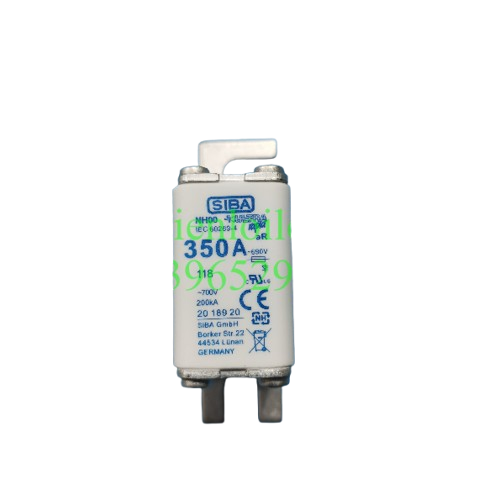
\includegraphics[width=0.3\textwidth]{pictures/2g.png}
                            \caption{Cầu chì SIBA NH00 350A}
                        \end{figure}
                    \item Thông số kỹ thuật cầu chì:
                        \begin{itemize}
                            \item Thương hiệu: SIBA.
                            \item Dòng định mức: 350A.
                            \item Dòng ngắn mạch: 200kA.
                            \item Báo trạng thái ngắt mạch: Có.
                            \item Đường dẫn sản phẩm: \href{https://thietbidienloiloidat.com/san-pham/cau-chi-siba-nh00-350a/}{Cầu chì SIBA}.
                        \end{itemize}
                \end{itemize}
        \subsubsection{Lamb}
            \textbf{Điều kiện chọn đèn}
                \begin{itemize}
                    \item Chọn đèn có điện áp làm việc $U = 220V$.
                    \item Chọn đèn có các màu tượng trưng cho các chức năng:
                        \begin{itemize}
                            \item Đỏ: Báo lỗi, cảnh báo nguy hiểm.
                            \item Xanh lá cây: Hoạt động bình thường.
                            \item Vàng (hoặc cam): Báo trạng thái chờ, chuẩn bị hoạt động.
                            \item Xanh dương: Báo tín hiệu đặc biệt (thường là trạng thái thủ công).
                            \item Trắng: Báo nguồn hoặc trạng thái trung tính.
                        \end{itemize}
                    \item Chọn đèn có công suất nhỏ (0.5W - 3W) để tiết kiệm năng lượng.
                \end{itemize}
            \begin{figure}[H]
                \centering
                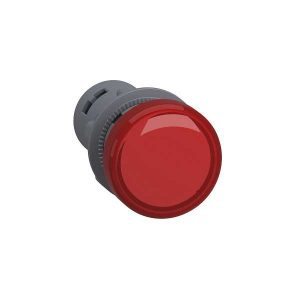
\includegraphics[width=0.2\textwidth]{pictures/2i.png}
                \caption{Đèn báo Schneider đỏ XA2EVM4LC, 22mm 220V AC}
            \end{figure}
            \begin{figure}[H]
                \centering
                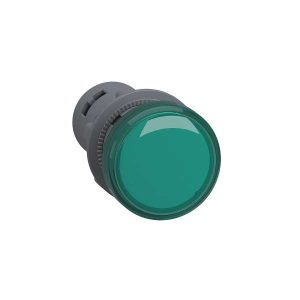
\includegraphics[width=0.2\textwidth]{pictures/2j.png}
                \caption{Đèn báo Schneider xanh XA2EVM3LC, 22mm 220V AC}
            \end{figure}
            \begin{figure}[H]
                \centering
                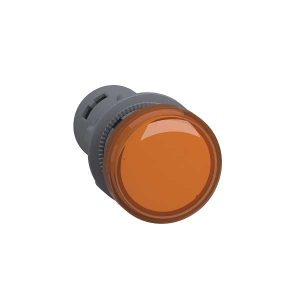
\includegraphics[width=0.2\textwidth]{pictures/2k.png}
                \caption{Đèn báo Schneider cam XA2EVM5LC, 22mm 220V AC}
            \end{figure}
        \subsubsection{Aptomat và dây dẫn}
            \textbf{Điều kiện chọn aptomat}
                \begin{itemize}
                    \item Chọn aptomat theo pha của nguồn cấp.
                    \item $I_{B} < I_{n} < I_{Z}$.
                    \item $I_{CSB} > I_{SC}$.\\[0.2cm]
                    Trong đó:
                    \begin{itemize}
                        \item $I_{B}$ là dòng điện tải lớn nhất.
                        \item $I_{n}$ dòng điện định mức của MCB, MCCB.
                        \item $I_{Z}$ dòng điện cho phép lớn nhất của dây dẫn điện .
                        \item $I_{CSB}$ là dòng điện lớn nhất mà MCB, MCCB có thể cắt.
                        \item $I_{SC}$ là dòng ngắn mạch của tải.
                    \end{itemize}
                \end{itemize}
            \textbf{Điều kiện chọn dây dẫn}
                \begin{figure}[H]
                    \centering
                    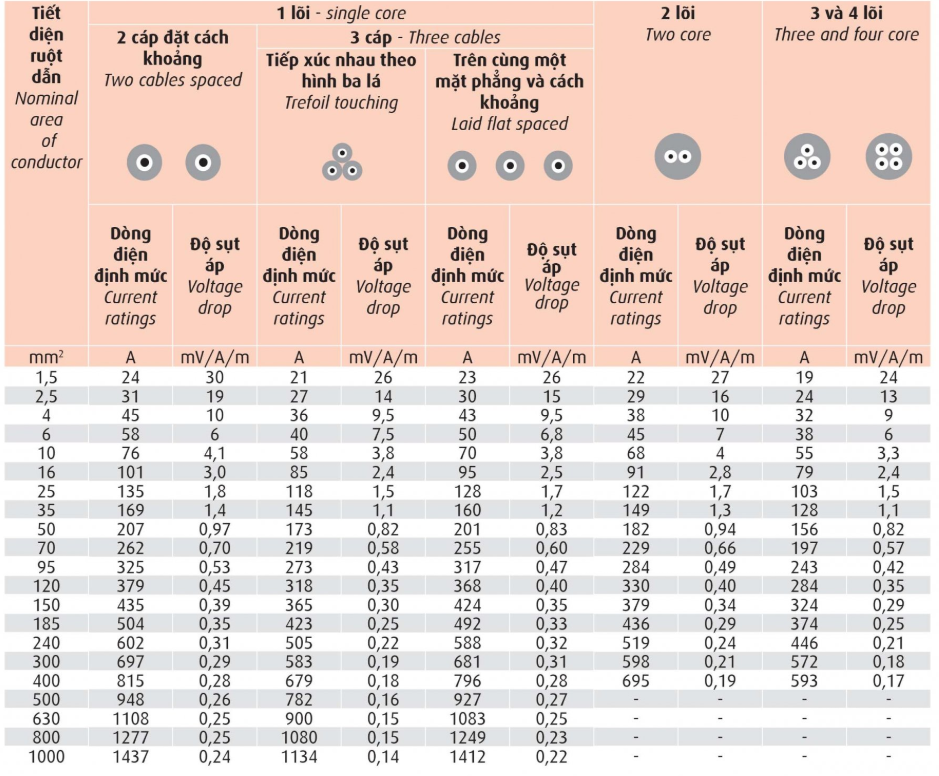
\includegraphics[width=1\textwidth]{pictures/2h.png}
                    \caption{Bảng chọn dây dẫn Cadivi}
                \end{figure}
            Giả sử $I_{CSB} > I_{SC}$ là điều kiện luôn thỏa. \\[0.2cm]
            \textbf{Chọn aptomat và dây dẫn cho tải 1}
                \begin{itemize}
                    \item Chọn aptomat MCCB LS ABN203c 200A 3P 30kA và dây dẫn Cadivi $50mm^2$ có dòng cho phép lớn nhất là $207A$.
                    \item Thông số kỹ thuật aptomat:
                        \begin{itemize}
                            \item Thương hiệu: LS.
                            \item Dòng định mức: 200A.
                            \item Dòng ngắn mạch: 30kA.
                            \item Điện áp ngõ vào: 3 pha
                            \item Series: LS ABN.
                            \item Đường dẫn sản phẩm: \href{https://codienhaiau.com/product/mccb-ls-abn203c-200a-30ka-3p/}{MCCB LS}.
                        \end{itemize}
                        \begin{figure}[H]
                            \centering
                            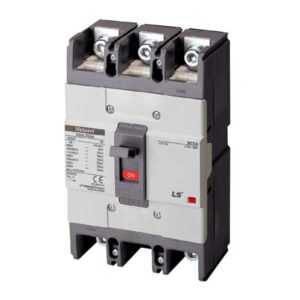
\includegraphics[width=0.4\textwidth]{pictures/2l.png}
                            \caption{MCCB LS ABN203c 200A 3P 30kA}
                        \end{figure}
                \end{itemize}
            \textbf{Chọn aptomat và dây dẫn cho tải 2}
                \begin{itemize}
                    \item Chọn aptomat MCCB Siemens 3VM1110-4ED12-0AA0 100A 36kA 1P và dây dẫn Cadivi $25mm^2$ có dòng cho phép lớn nhất là $135A$.
                    \item Thông số kỹ thuật aptomat:
                        \begin{itemize}
                            \item Thương hiệu: Siemens.
                            \item Dòng định mức: 100A.
                            \item Dòng ngắn mạch: 36kA.
                            \item Điện áp ngõ vào: 1 pha.
                            \item Series: Siemens 3VM.
                            \item Đường dẫn sản phẩm: \href{https://codienhaiau.com/product/mccb-siemens-3vm1110-4ed12-0aa0-100a-36ka-1p/}{MCCB Siemens}.
                        \end{itemize}
                        \begin{figure}[H]
                            \centering
                            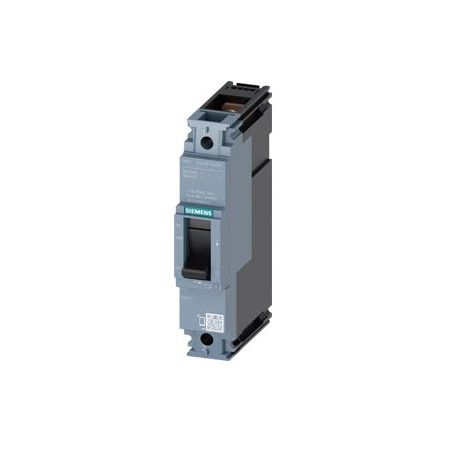
\includegraphics[width=0.4\textwidth]{pictures/2m.png}
                            \caption{MCCB Siemens 3VM1110-4ED12-0AA0 100A 36kA 1P}
                        \end{figure}
                \end{itemize}
            \textbf{Chọn aptomat và dây dẫn cho tải 3}
                \begin{itemize}
                    \item Chọn aptomat MCCB LS ABN203c 225A 3P 30kA và dây dẫn Cadivi $70mm^2$ có dòng cho phép lớn nhất là $321A$.
                    \item Thông số kỹ thuật aptomat:
                        \begin{itemize}
                            \item Thương hiệu: LS.
                            \item Dòng định mức: 225A.
                            \item Dòng ngắn mạch: 30kA.
                            \item Điện áp ngõ vào: 3 pha.
                            \item Series: LS ABN.
                            \item Đường dẫn sản phẩm: \href{https://codienhaiau.com/product/mccb-ls-abn203c-225a-30ka-3p/}{MCCB LS}.
                        \end{itemize}
                        \begin{figure}[H]
                            \centering
                            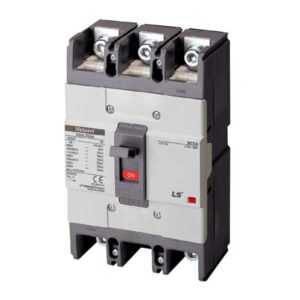
\includegraphics[width=0.4\textwidth]{pictures/2n.png}
                            \caption{MCCB LS ABN203c 225A 3P 30kA}
                        \end{figure}
                \end{itemize}
                
                
    
                
            
            
\end{document}